% Model-derived trajectories: panel (a) is the exact two-pulse flow;
% panel (b) samples the Appendix D N=10 full-coverage construction.
% The latter's numerical direction and cut times are regenerated by
% verification/twin_ten_asset_benchmarks.py (not an interval certificate).
\begin{figure}[tbp]
\centering
\resizebox{0.98\linewidth}{!}{%
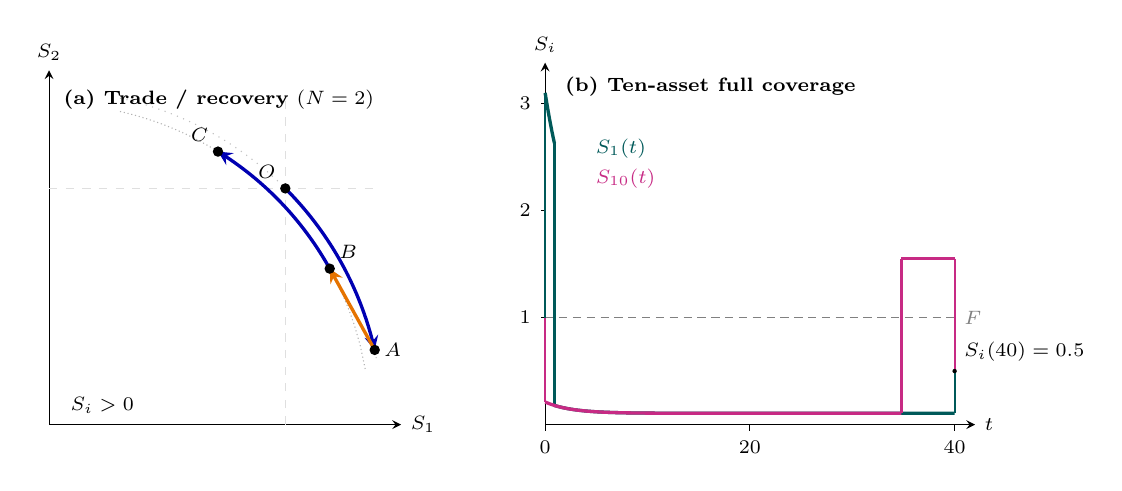
\begin{tikzpicture}[font=\scriptsize,>=stealth]
\pgfmathsetmacro{\sA}{sqrt(1.9)}
\pgfmathsetmacro{\sB}{sqrt(0.1)}
\pgfmathsetmacro{\sC}{1+(\sA-1)*exp(-0.7)}
\pgfmathsetmacro{\sD}{1+(\sB-1)*exp(-0.7)}
\pgfmathsetmacro{\rB}{\sC*\sC+\sD*\sD}
\pgfmathsetmacro{\sE}{sqrt(\sC*\sC-0.9)}
\pgfmathsetmacro{\sF}{sqrt(\sD*\sD+0.9)}
% (a) N=2, F=eta=rho=1: trade h=0.45, recover 0.7, reverse h.
\begin{scope}[x=3.0cm,y=3.0cm]
  \draw[->] (0,0) -- (1.49,0) node[right] {$S_1$};
  \draw[->] (0,0) -- (0,1.5) node[above] {$S_2$};
  \draw[gray!25,dashed] (1,0) -- (1,1.38);
  \draw[gray!25,dashed] (0,1) -- (1.4,1);
  \draw[gray!50,dotted,domain=0.30:1.39,samples=45]
    plot ({\x},{sqrt(2-\x*\x)});
  \draw[gray!60,densely dotted,domain=0.30:1.34,samples=45]
    plot ({\x},{sqrt(\rB-\x*\x)});
  \draw[blue!70!black,very thick,domain=0:0.45,samples=40,->]
    plot ({sqrt(1+2*\x)},{sqrt(1-2*\x)});
  \draw[orange!90!black,very thick,domain=0:0.7,samples=45,->]
    plot ({1+(\sA-1)*exp(-\x)},{1+(\sB-1)*exp(-\x)});
  \draw[blue!70!black,very thick,domain=0:0.45,samples=45,->]
    plot ({sqrt(\sC*\sC-2*\x)},{sqrt(\sD*\sD+2*\x)});
  \fill (1,1) circle (0.022) node[above left] {$O$};
  \fill (\sA,\sB) circle (0.022) node[right] {$A$};
  \fill (\sC,\sD) circle (0.022) node[above right] {$B$};
  \fill (\sE,\sF) circle (0.022) node[above left] {$C$};
  \node[anchor=north west] at (0.02,1.46)
    {\textbf{(a) Trade / recovery} ($N=2$)};
  \node[anchor=west] at (0.05,0.08) {$S_i>0$};
\end{scope}
% (b) N=10, F=eta=1, rho=.4, T=40, full-coverage Appendix D.
% R(t)=H+(sqrt(10)-H) exp(-.4t), directions (a,b,...,b).
\begin{scope}[shift={(6.3cm,0)},x=0.13cm,y=1.36cm]
  \draw[->] (0,0) -- (42,0) node[right] {$t$};
  \draw[->] (0,0) -- (0,3.38) node[above] {$S_i$};
  \draw[densely dashed,gray] (0,1) -- (40,1) node[right] {$F$};
  \foreach \t in {0,20,40}{
    \draw (\t,0) -- (\t,-0.06) node[below] {\t};
  }
  \foreach \p in {1,2,3}{
    \draw (0,\p) -- (-0.45,\p) node[left] {\p};
  }
  \pgfmathsetmacro{\a}{0.9796977322918206}
  \pgfmathsetmacro{\b}{0.0668267688731795}
  \pgfmathsetmacro{\h}{1.5811386521504363}
  \pgfmathsetmacro{\d}{sqrt(10)-\h}
  \draw[teal!70!black,thick] (0,1) -- (0,{sqrt(10)*\a});
  \draw[teal!70!black,very thick,domain=0:0.90218336,samples=12]
    plot (\x,{\a*(\h+\d*exp(-0.4*\x))});
  \draw[teal!70!black,thick]
    (0.90218336,{\a*(\h+\d*exp(-0.4*0.90218336))}) --
    (0.90218336,{\b*(\h+\d*exp(-0.4*0.90218336))});
  \draw[teal!70!black,very thick,domain=0.90218336:40,samples=100]
    plot (\x,{\b*(\h+\d*exp(-0.4*\x))});
  \draw[teal!70!black,thick]
    (40,{\b*(\h+\d*exp(-0.4*40))}) -- (40,0.5);
  \draw[magenta!80!black,thick] (0,1) -- (0,{sqrt(10)*\b});
  \draw[magenta!80!black,very thick,domain=0:34.80222557,samples=100]
    plot (\x,{\b*(\h+\d*exp(-0.4*\x))});
  \draw[magenta!80!black,thick]
    (34.80222557,{\b*(\h+\d*exp(-0.4*34.80222557))}) --
    (34.80222557,{\a*(\h+\d*exp(-0.4*34.80222557))});
  \draw[magenta!80!black,very thick,domain=34.80222557:40,samples=30]
    plot (\x,{\a*(\h+\d*exp(-0.4*\x))});
  \draw[magenta!80!black,thick]
    (40,{\a*(\h+\d*exp(-0.4*40))}) -- (40,0.5);
  \fill (40,0.5) circle (0.8pt) node[above right] {$S_i(40)=0.5$};
  \node[anchor=north west] at (1,3.34)
    {\textbf{(b) Ten-asset full coverage}};
  \node[teal!70!black,anchor=west] at (4,2.58) {$S_1(t)$};
  \node[magenta!80!black,anchor=west] at (4,2.30) {$S_{10}(t)$};
\end{scope}
\end{tikzpicture}%
}
\caption{\textbf{Conservation geometry and resilience-driven reachability.}
(a) Under constant impact $g=1$ with $N=2$ and $F=\rho=1$, equal-and-opposite
paired-dollar pulses of magnitude $0.45$ follow the distinct fixed-radius
curves $O\to A$ and $B\to C$; recovery over $T=0.7$ moves the state
from $A$ to $B$ and changes the conserved radius. Both individual executed-dollar
ledgers close, yet $C\ne O$ and the mean log loss is positive.
(b) Selected prices in the analytical ten-asset full-coverage witness with
$\rho=0.4$ and $T=40$; the other eight assets take the same cyclic high
and low roles. Flow-completed pulses produce the jumps. All ten prices
finish at $F/2$ with $X_i(40)=0$. Both panels stay at strictly positive
prices and represent exact model paths evaluated numerically, not
observed prices or new interval certificates.}
\label{fig:conservation-geometry}
\end{figure}
